\def\year{2022}\relax
%File: formatting-instructions-latex-2022.tex
%release 2022.1
\documentclass[letterpaper]{article} % DO NOT CHANGE THIS
\usepackage{aaai22}  % DO NOT CHANGE THIS
\usepackage{times}  % DO NOT CHANGE THIS
\usepackage{helvet}  % DO NOT CHANGE THIS
\usepackage{courier}  % DO NOT CHANGE THIS
\usepackage[hyphens]{url}  % DO NOT CHANGE THIS
\usepackage{graphicx} % DO NOT CHANGE THIS
\urlstyle{rm} % DO NOT CHANGE THIS
\def\UrlFont{\rm}  % DO NOT CHANGE THIS
\usepackage{natbib}  % DO NOT CHANGE THIS AND DO NOT ADD ANY OPTIONS TO IT
\usepackage{caption} % DO NOT CHANGE THIS AND DO NOT ADD ANY OPTIONS TO IT
\DeclareCaptionStyle{ruled}{labelfont=normalfont,labelsep=colon,strut=off} % DO NOT CHANGE THIS
\frenchspacing  % DO NOT CHANGE THIS
\setlength{\pdfpagewidth}{8.5in}  % DO NOT CHANGE THIS
\setlength{\pdfpageheight}{11in}  % DO NOT CHANGE THIS
%
% These are recommended to typeset algorithms but not required. See the subsubsection on algorithms. Remove them if you don't have algorithms in your paper.
\usepackage{algorithm}
\usepackage{algorithmic}

%
% These are are recommended to typeset listings but not required. See the subsubsection on listing. Remove this block if you don't have listings in your paper.
\usepackage{newfloat}
\usepackage{listings}
\lstset{%
	basicstyle={\footnotesize\ttfamily},% footnotesize acceptable for monospace
	numbers=left,numberstyle=\footnotesize,xleftmargin=2em,% show line numbers, remove this entire line if you don't want the numbers.
	aboveskip=0pt,belowskip=0pt,%
	showstringspaces=false,tabsize=2,breaklines=true}
\floatstyle{ruled}
\newfloat{listing}{tb}{lst}{}
\floatname{listing}{Listing}
%
%\nocopyright
%
% PDF Info Is REQUIRED.
% For /Title, write your title in Mixed Case.
% Don't use accents or commands. Retain the parentheses.
% For /Author, add all authors within the parentheses,
% separated by commas. No accents, special characters
% or commands are allowed.
% Keep the /TemplateVersion tag as is
\pdfinfo{
/Title (AAAI Press Formatting Instructions for Authors Using LaTeX -- A Guide)
/Author (AAAI Press Staff, Pater Patel Schneider, Sunil Issar, J. Scott Penberthy, George Ferguson, Hans Guesgen, Francisco Cruz, Marc Pujol-Gonzalez)
/TemplateVersion (2022.1)
}

% DISALLOWED PACKAGES
% \usepackage{authblk} -- This package is specifically forbidden
% \usepackage{balance} -- This package is specifically forbidden
% \usepackage{color (if used in text)
% \usepackage{CJK} -- This package is specifically forbidden
% \usepackage{float} -- This package is specifically forbidden
% \usepackage{flushend} -- This package is specifically forbidden
% \usepackage{fontenc} -- This package is specifically forbidden
% \usepackage{fullpage} -- This package is specifically forbidden
% \usepackage{geometry} -- This package is specifically forbidden
% \usepackage{grffile} -- This package is specifically forbidden
% \usepackage{hyperref} -- This package is specifically forbidden
% \usepackage{navigator} -- This package is specifically forbidden
% (or any other package that embeds links such as navigator or hyperref)
% \indentfirst} -- This package is specifically forbidden
% \layout} -- This package is specifically forbidden
% \multicol} -- This package is specifically forbidden
% \nameref} -- This package is specifically forbidden
% \usepackage{savetrees} -- This package is specifically forbidden
% \usepackage{setspace} -- This package is specifically forbidden
% \usepackage{stfloats} -- This package is specifically forbidden
% \usepackage{tabu} -- This package is specifically forbidden
% \usepackage{titlesec} -- This package is specifically forbidden
% \usepackage{tocbibind} -- This package is specifically forbidden
% \usepackage{ulem} -- This package is specifically forbidden
% \usepackage{wrapfig} -- This package is specifically forbidden
% DISALLOWED COMMANDS
% \nocopyright -- Your paper will not be published if you use this command
% \addtolength -- This command may not be used
% \balance -- This command may not be used
% \baselinestretch -- Your paper will not be published if you use this command
% \clearpage -- No page breaks of any kind may be used for the final version of your paper
% \columnsep -- This command may not be used
% \newpage -- No page breaks of any kind may be used for the final version of your paper
% \pagebreak -- No page breaks of any kind may be used for the final version of your paperr
% \pagestyle -- This command may not be used
% \tiny -- This is not an acceptable font size.
% \vspace{- -- No negative value may be used in proximity of a caption, figure, table, section, subsection, subsubsection, or reference
% \vskip{- -- No negative value may be used to alter spacing above or below a caption, figure, table, section, subsection, subsubsection, or reference

\setcounter{secnumdepth}{0} %May be changed to 1 or 2 if section numbers are desired.

% The file aaai22.sty is the style file for AAAI Press
% proceedings, working notes, and technical reports.
%

% Title

% Your title must be in mixed case, not sentence case.
% That means all verbs (including short verbs like be, is, using,and go),
% nouns, adverbs, adjectives should be capitalized, including both words in hyphenated terms, while
% articles, conjunctions, and prepositions are lower case unless they
% directly follow a colon or long dash
\title{Towards a robot partner reducing\\ ambiguities using perspective taking}
\author{
    %Authors
    % All authors must be in the same font size and format.
    Anthony Favier\textsuperscript{\rm 1,2},
    Shashank Shekhar\textsuperscript{\rm 1},
    Rachid Alami\textsuperscript{\rm 1,2}
}
\affiliations{
    %Afiliations
    \textsuperscript{\rm 1}LAAS-CNRS, Universite de Toulouse, CNRS, Toulouse, France\\
    \textsuperscript{\rm 2}{Artificial and Natural Intelligence Toulouse Institute (ANITI)}

    % email address must be in roman text type, not monospace or sans serif
    \{anthony.favier, sshekhar, rachid.alami\}@laas.fr
}

\begin{document}

%%%%% SYMBOLS DEFINITION %%%%%
\newcommand{\worldstates}{\mathcal{S}}
\newcommand{\worldstate}{s}
\newcommand{\fluent}[3]{\mathcal{F}^{#1#2}_{#3}}
\newcommand{\prop}{\varphi}
\newcommand{\allprops}{\Phi}
\newcommand{\predicate}{\mathcal{P}}
\newcommand{\predval}{v}
\newcommand{\agent}{\lambda}
\newcommand{\beliefs}{\mathcal{B}}
\newcommand{\human}{H}
\newcommand{\robot}{R}
\newcommand{\places}{\mathcal{P}}
\newcommand{\place}{p}
\newcommand{\unknown}{UnKw}
\newcommand{\known}{Kw}
\newcommand{\missedactions}{\mathcal{M}}
\newcommand{\loc}[1]{loc(#1)}
\newcommand{\obs}[1]{obs(#1)}
\newcommand{\dom}[1]{dom(#1)}
\newcommand{\observable}{\texttt{OBS}}
\newcommand{\inferrable}{\texttt{INF}}
%%%%%%%%%%%%%%%%%%%%%%%%%%%%%%

\maketitle

\begin{abstract}
\end{abstract}

\section{Introduction}
% what is known ? our understanding of the world
general context, towards robot partner. 

% what is unknown ? the gap we want to fill
% how and why ? your rational and purpose/hypothesis 

\clearpage
\section{Materials and Methods}
% what did you do ?

The work \cite{buisan:hal-03684211} already support collaborative task planning while maintaining distinct beliefs/knowledge for each agent. Based on this work, we enhanced the task planner with a few concept linked to perspective taking and observability in order to reduce the ambiguities that may happen in a collaborative task. First we predict the situation assessment of an agent. On the other hand, we look for belief divergences that have a detrimental influence on the plan in order to fix them with communication. We also check observability of action execution to update beliefs with different types of effects.

\subsection{Knowledge representation definitions}

Our formalism is close to the SAS+ Formalism applied to HTN.  

\begin{itemize}

    \item \textbf{Word state}: Let $\worldstates$ be the set of all possible world states, any world state is composed of a set of multi-valued state variable that we call fluents, i.e. $\forall\worldstate\in\worldstates, \worldstate=\{ \fluent{\worldstate}{}{}{} \}$.
    
    \item \textbf{Fluent}: A fluent $\fluent{\worldstate}{}{}{}$ is a statement partially describing a world state $\worldstate\in\worldstates$ whose truth value is situation dependent. Fluents may be seen as ''properties of the world" that may change over time.
    \subitem E.g. Considering the fluent $\fluent{\worldstate}{}{at}{, ball} \equiv at(ball, \worldstate)$, if the ball is initially in $place_1$ then $\fluent{\worldstate_0}{}{at}{,ball}=place_1$, $\worldstate_0$ being the initial state.
 
    
    \item \textbf{Belief divergence}: We note $\fluent{\worldstate}{,\agent}{}{}$ a fluent evaluated in the perspective of an agent $\agent$. Thus, for a given real state of the world $\worldstate\in\worldstates$, the robot and the human can have different values for the same fluent. We call such mismatch a belief divergence.
    \subitem E.g. $(\fluent{\worldstate_0}{,\robot}{at}{,ball}=place_1) \neq (\fluent{\worldstate_0}{,\human}{at}{,ball}=place_2)$
    
    \item \textbf{Beliefs}: We call beliefs of an agent $\agent$, noted $\beliefs_\agent$, the state $\worldstate_\agent\in\worldstates$ in which this agent thinks the world is in, i.e. the set of all fluents evaluated in their perspective: $\worldstate_\agent=\{ \fluent{\worldstate}{,\agent}{}{} \}$. It is important to note that the beliefs of the robot $\beliefs_\robot$ are assumed to be the ground truth, as we consider the planner as being part of the robot. Note also that the human's beliefs $\beliefs_\human$ are only estimated by the robot by doing some perspective-taking reasoning.
    
\end{itemize}

\subsection{Observability definitions and processes}

\begin{itemize}

    \item \textbf{Action effects}: 
    Actions can have three types of effects: 
    \subitem - \textbf{non-observable}: Effects that can't be observed by other agents.
    \subitem - \textbf{inferable}: Effects that can't be observed but can be inferred by agents observing the action execution.
    \subitem - \textbf{observable}: Effects that can be observed by other agents, regardless if the action execution has been observed.
    
    \item \textbf{Places}: 
    A place is an area in the environment. Let $\places=\{ \place_i \}$ be the set of all defined places. Agents are always situated in a place. Actions are always performed in a place, except for navigation actions that involve two places.

\end{itemize}    

\begin{itemize}

    \item \textbf{Observation of an action execution}: 
    For simplification purposes we define the notion of co-presence. Two agents located in a same place are said to be co-present.
    Based on that, we assume that the execution of an action being performed by an agent $\agent$ is observed by all agents that were co-present with $\agent$ either at the before or after the action.
    The co-presence is checked both before and after to cover navigation actions.
    As future work a more elaborated formula could be used to evaluate the observation of an action execution, for instance using geometrical reasoning.
    
    \item \textbf{Checking observability when executing an action}: 
    Consider two agents $\lambda_1$ and $\lambda_2$. When $\agent_1$ performs an action, we first update the acting agent's beliefs $\beliefs_{\agent_1}$ with all the effects of the action. Then, before updating the other agent's beliefs $\beliefs_{\agent_2}$, we check if $\agent_2$ observed the action execution of $\agent_1$. 
    To do so, according to our assumption, we simply check if $\agent_1$ and $\agent_2$ were co-present either before or after simulating the action's effects. If so, $\agent_2$ observed the action execution and $\beliefs_{\agent_2}$ is updated with both the inferable and observable effects. 
    Otherwise, the action missed by $\agent_2$ is stored in a set noted $\missedactions_{\agent_2}$, which stores every actions missed by $\agent_2$.
    
    \item \textbf{Situation Assessment}: 
    The idea is to predict the situation assessment of an agent and update their beliefs about all the observable effects that they missed while being away. 
    To do so, when an agent $\agent$ enters a place $\place\in\places$, all the non observed actions that happened in $\place$ are extracted from $\missedactions_\agent$. Then, we chronologically apply the effects of each of these actions and remove them from $\missedactions_\agent$. If $\agent$ is the robot, all the effects are applied. Otherwise, if $\agent$ is the human, only the observable effects are applied. 
    
    \item \textbf{Checking if there are relevant false beliefs}: 
    We want to detect if a false belief influences the plan of the human, i.e. if when using the human beliefs containing false beliefs induces different human actions than the ones expected using the ground truth beliefs. If so, the false beliefs are qualified as relevant. Indeed, a false belief can wrongly affect the applicability of a human action, its cost and its effects. Assuming that the robot estimated the best possible plans for the human using the ground truth $\beliefs_\robot$, any different plan found with $\beliefs_\human$ is either not applicable in reality, more expensive or with undesired effects. Thus, a relevant false belief is always considered as detrimental.

    When refining the human agenda to estimate their next possible actions, we first use the human beliefs $\beliefs_H$. Then we repeat the process but considering the robot beliefs $\beliefs_R$ (ground truth). After, the two obtained refinements are compared to check if they are the same. Two refinements are considered to be the same if they respectively have the same decompositions, i.e. if, in both refinements, each decomposition respectively has the same type, subtasks and if their actions have the same applicability, cost and effects. If the two refinements are not the same we consider that there are relevant belief divergences to align, but we don't know which ones yet.
    
    \item \textbf{Identify the relevant false beliefs and communicate}: 
    Once the presence of relevant false beliefs has been confirmed they have to be identified. For now, all divergences between $\mathcal{B}_R$ and $\mathcal{B}_H$ are first computed. Then one divergence after another we simulate the divergence correction (i.e. $ \fluent{\worldstate}{,\human}{i}{} \gets \fluent{\worldstate}{,\robot}{i}{}$) and the human agenda is refined again in order to compare the new refinement with the one previously obtained with $\beliefs_\robot$. We keep simulating combination of divergence corrections until the refinements are the same, which means that all the relevant false beliefs have been identified. Then, the corresponding communication action is inserted in the robot's plan to inform the human about their relevant false beliefs and to correct them.
    
    Communication actions are supposed to be instantaneous (0 time step to execute) and for now are inserted right before the detected erroneous human action.
    
\end{itemize}

\subsection{Choice to reduce ambiguities when relevant false belief}
% Quick notes about choice to communicate to reduce ambiguities (ONLY when there is a relevant false belief) (because even if there is a relevant false belief, the human is rational and will rarely perform a shared task without questioning their partner who might have done it already) 
In the case of a shared goal, assume that the human didn't observe the robot performing an action with only inferable effects, that meaning the when coming back to the robot the human has no way to tell the action has been done by looking at the scene. Then three cases can occur : 1) The human considers that the robot didn't perform the action, thus the human will try to perform it again, 2) The human considers that the robot performed the action so the plan execution continues, 3) the human prefers to directly ask the robot if it performed the action. No matter which case we are in when the human is back, there is an ambiguity, the human can't be sure about the action execution so they can either assume the robot did or didn't do it, either directly ask the robot. Even though in some situations the action execution can be inferred (e.g. we observe the effect of an following action, thus the prior actions to this observable one must have been executed), we consider that there will always be an ambiguity. Hence, even if in some situations the human guessed right or asked (will rarely perform again) we decide to communicate anyway to proactively reduce ambiguities in the plan. Again, this communication could be optional in some situations (thus plan with less steps) but having a plan without ambiguities is better than a plan with less steps but where agent aren't sure about what they have to do. Communication help to compel the human actions.


for now purely symbolic reasoning, for both action execution and action effects observability. But we can imagine geometric reasoning for those both.

\section{Results}
% what results did you get ?

Present example : Probably cooking example turning fire (situation assessment) and adding salt (relevant divergence). Show plan without our contribution. Then show what we obtain with our contribution.



Think about other configuration of the same scenario for other cases ? Here prevent action with undesired effects. Should find also applicability and cost.

Quantitative: We can randomize or use all combination of initial state : pasta location, starting agent, initial agent location, (initial belief divergence ?). Make statistics on applicability of plans with and withou contribution 

Qualitative :

For these examples, the world state is composed of the following fluents :\\
- $\fluent{\worldstate}{}{salt}{} \equiv salt\_added(s)\in\{true, false\}$\\
- $\fluent{\worldstate}{}{fire}{} \equiv pot\_fire\_on(s)\in\{true, false\}$\\
- $\fluent{\worldstate}{}{at}{, \{\robot,\human,pasta\} } \equiv at(e, s)\in \{place_1, place_2\}$
% , e \in \{ \robot, \human, pasta \}$

\begin{figure}
    \centering
    \includegraphics[width=\linewidth]{figures/example.png}
    \caption{Scene cooking}
    \label{fig:scene}
\end{figure}

Task description in HTN depicted in Fig.~\ref{fig:htn}

\begin{figure}
    \centering
    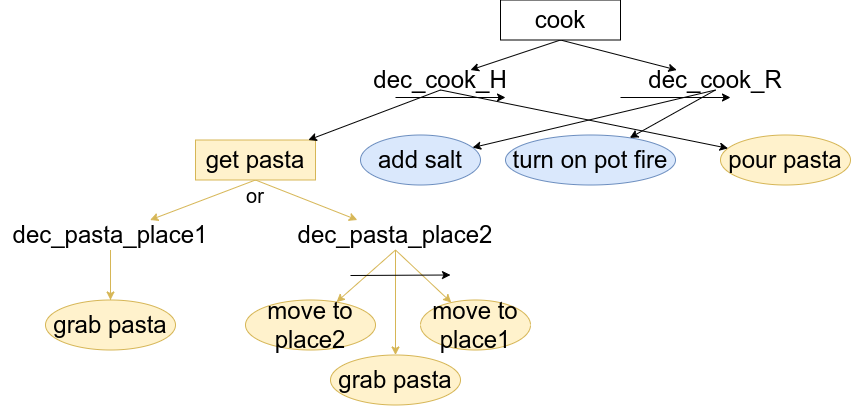
\includegraphics[width=\linewidth]{figures/htn.png}
    \caption{HTN, cook task description}
    \label{fig:htn}
\end{figure}

\begin{figure*}
    \centering
    \includegraphics[width=\linewidth]{figures/htn_cook_example.drawio.png}
    \caption{Caption}
    \label{fig:scenarios}
\end{figure*}







Scenarios:
\begin{itemize}
    \item \textbf{pasta in same place}
        \subitem normal execution
    
    \item \textbf{pasta in another place, R starts}
        \subitem w/o: Agents are omniscient, H knows instantly about the effects of R actions even without observing the actions
        \subitem w/: H sees salt action and assess the fire on action when coming back. Thus no com required, same plan than w/o but beliefs have been updated differently
        
    \item \textbf{pasta in another place, H starts}
        \subitem w/o: Agents omniscient again, H knows about all R actions instantly
        \subitem w/: R predicts H will miss both actions but will be able to assess the pot fire action execution when back in place1 but can't be sure about salt action. Decides to com to remove ambiguitiy
    
    \item \textbf{initial belief divergence on pasta location(R:place1 H:place2). The robot brought the pasta closer before the human comes}
        \subitem w/o: Plan isn't actually applicable with ground truth knowledge (grab pasta, no pasta here)
        \subitem w/: Relevant belief divergence detected. R com to correct the relevant divergence and make H plan applicable
    
    
\end{itemize}

\section{Discussion}
% how do the results fill the gap ?

Point out ambiguities (created both by the lack of situation assessment and belief alignment) in the plans without contribution. Then, explain how we removed them. 

\section{Conclusion}
% what does this mean for us going forward ?

\bibliography{bib.bib}

\end{document}
